\begin{tikzpicture}
	\visible<2>{
	\node[] () at (0,-0.2) {\begin{tikzpicture}[scale=0.62]
		\begin{axis}[
		%ticks=none,
		height=0.5\textwidth,
		width=0.1\textwidth,
		scale only axis,
		enlargelimits=false,
		axis on top,
		xlabel={Resistivity [$\Omega$m]},
		xtick={0,1.2,2.39},
		xticklabels={100,200,300},
		ytick={0.93,1.85,2.78,3.7,4.65,5.56,6.50,7.44,8.37,9.305,10.24,11.18,12.08,13},
		yticklabels={130,120,110,100,90,80,70,60,50,40,30,20,10,0},
		ylabel={Deep [m]},
		label style={font=\tiny},
		tick label style={font=\tiny}] 
		\addplot[thick] graphics[xmin=0,xmax=3,ymin=0,ymax=13] {Diapos/Intro/Figures/resis1};
		\end{axis}
		\end{tikzpicture}};
		}
		
	\node[] () at (4.3,0.2) {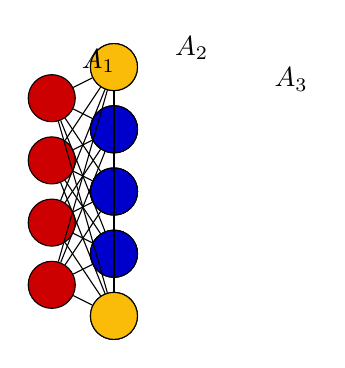
\begin{tikzpicture}[scale=0.79]
		\tikzstyle{every pin edge}=[<-,shorten <=1pt]
		\tikzstyle{neuron}=[circle,fill=black!25,minimum size=17pt,inner sep=0pt]
		\tikzstyle{input neuron}=[neuron,draw=black,fill=red!80!black];
		\tikzstyle{output neuron}=[neuron,draw=black,fill=blue!80!black];
		\tikzstyle{hidden neuron}=[neuron,draw=black,fill=yellow!50!orange];
		\tikzstyle{annot} = [text width=4em, text centered]
			
			% Draw the input layer nodes
		\foreach \name / \y in {1,...,4}
		% This is the same as writing \foreach \name / \y in {1/1,2/2,3/3,4/4}
		\node[input neuron] (I-\name) at (0,-\y) {};
			
			% Draw the hidden layer nodes
		\foreach \name / \y in {1,...,5}
		\path[yshift=0.5cm]
		node[hidden neuron] (H-\name) at (\layersep,-\y cm) {};
			
			% Draw the hidden layer nodes
		\foreach \name / \y in {1,...,5}
		\path[yshift=0.5cm]
		node[hidden neuron] (H2-\name) at (\layersep+\layersep,-\y cm) {};
			
			
			% Draw the output layer node
		\foreach \name / \y in {1,...,3}
		\path[yshift=-0.5cm]
		node[output neuron] (O-\name) at (\layersep+\layersep+\layersep,-\y cm) {};
			
			% Connect every node in the input layer with every node in the
			% hidden layer.
		\foreach \source in {1,...,4}
		\foreach \dest in {1,...,5}
		\path (I-\source) edge (H-\dest);
			
		\foreach \source in {1,...,5}
		\foreach \dest in {1,...,5}
		\path (H-\source) edge (H2-\dest);
			
			% Connect every node in the hidden layer with the output layer
		\foreach \source in {1,...,5}
		\foreach \dest in {1,...,3}
		\path (H2-\source) edge (O-\dest);

	    \node[] () at (0.75, -.4) {$A_1$};	
		\node[] () at (2.25, -0.2) {$A_2$};
		\node[] () at (3.85,-.7) {$A_3$};
			% Annotate the layers
		\end{tikzpicture}};
	\node[] () at (4.3, 2.8) {Neural Network};		
	\visible<2>{	
	\node[] () at (8.8, 1.2) {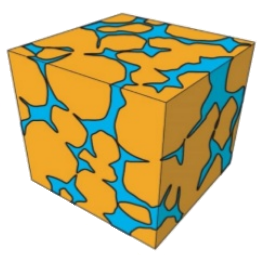
\includegraphics[width=2.5cm]{Diapos/Intro/Figures/res1}};
	\node[] () at (8.8,-1.4) {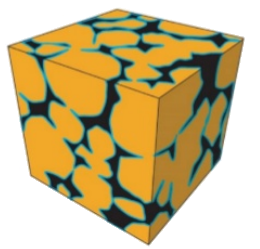
\includegraphics[width=2.5cm]{Diapos/Intro/Figures/res2}};
	\node[] () at (8.4, 2.8) {Output};
	\node[] () at (0.2, 2.8) {Input};
		
	\draw [decorate,very thick,decoration={brace,amplitude=10pt},xshift=-4pt,yshift=0pt]
		(1.3,2.8) -- (1.3,-2.4);
	\draw [decorate,very thick,decoration={brace,amplitude=10pt},xshift=-4pt,yshift=0pt]
		(7.5,-2.4) -- (7.5,2.8);
		
	\node[right] () at (9.0, 0.0) {\scriptsize Water};		
	\node[right] () at (9.0, -2.5) {\scriptsize Oil};	
	}			
\end{tikzpicture}